\section{Arrangements of Unbounded Curves\label{arr_sec:unbounded}}
%========================================

So far we have contstructed and manipulated only arrangements of
line segments, namely of bounded curves. Such arrangements always
have one unbounded face that contains all other arrangement features.
In this section we explain how to construct arrangements of unbounded
curves, being lines and rays in this context.

\begin{figure}[t]
\begin{ccTexOnly}
  \begin{center}
  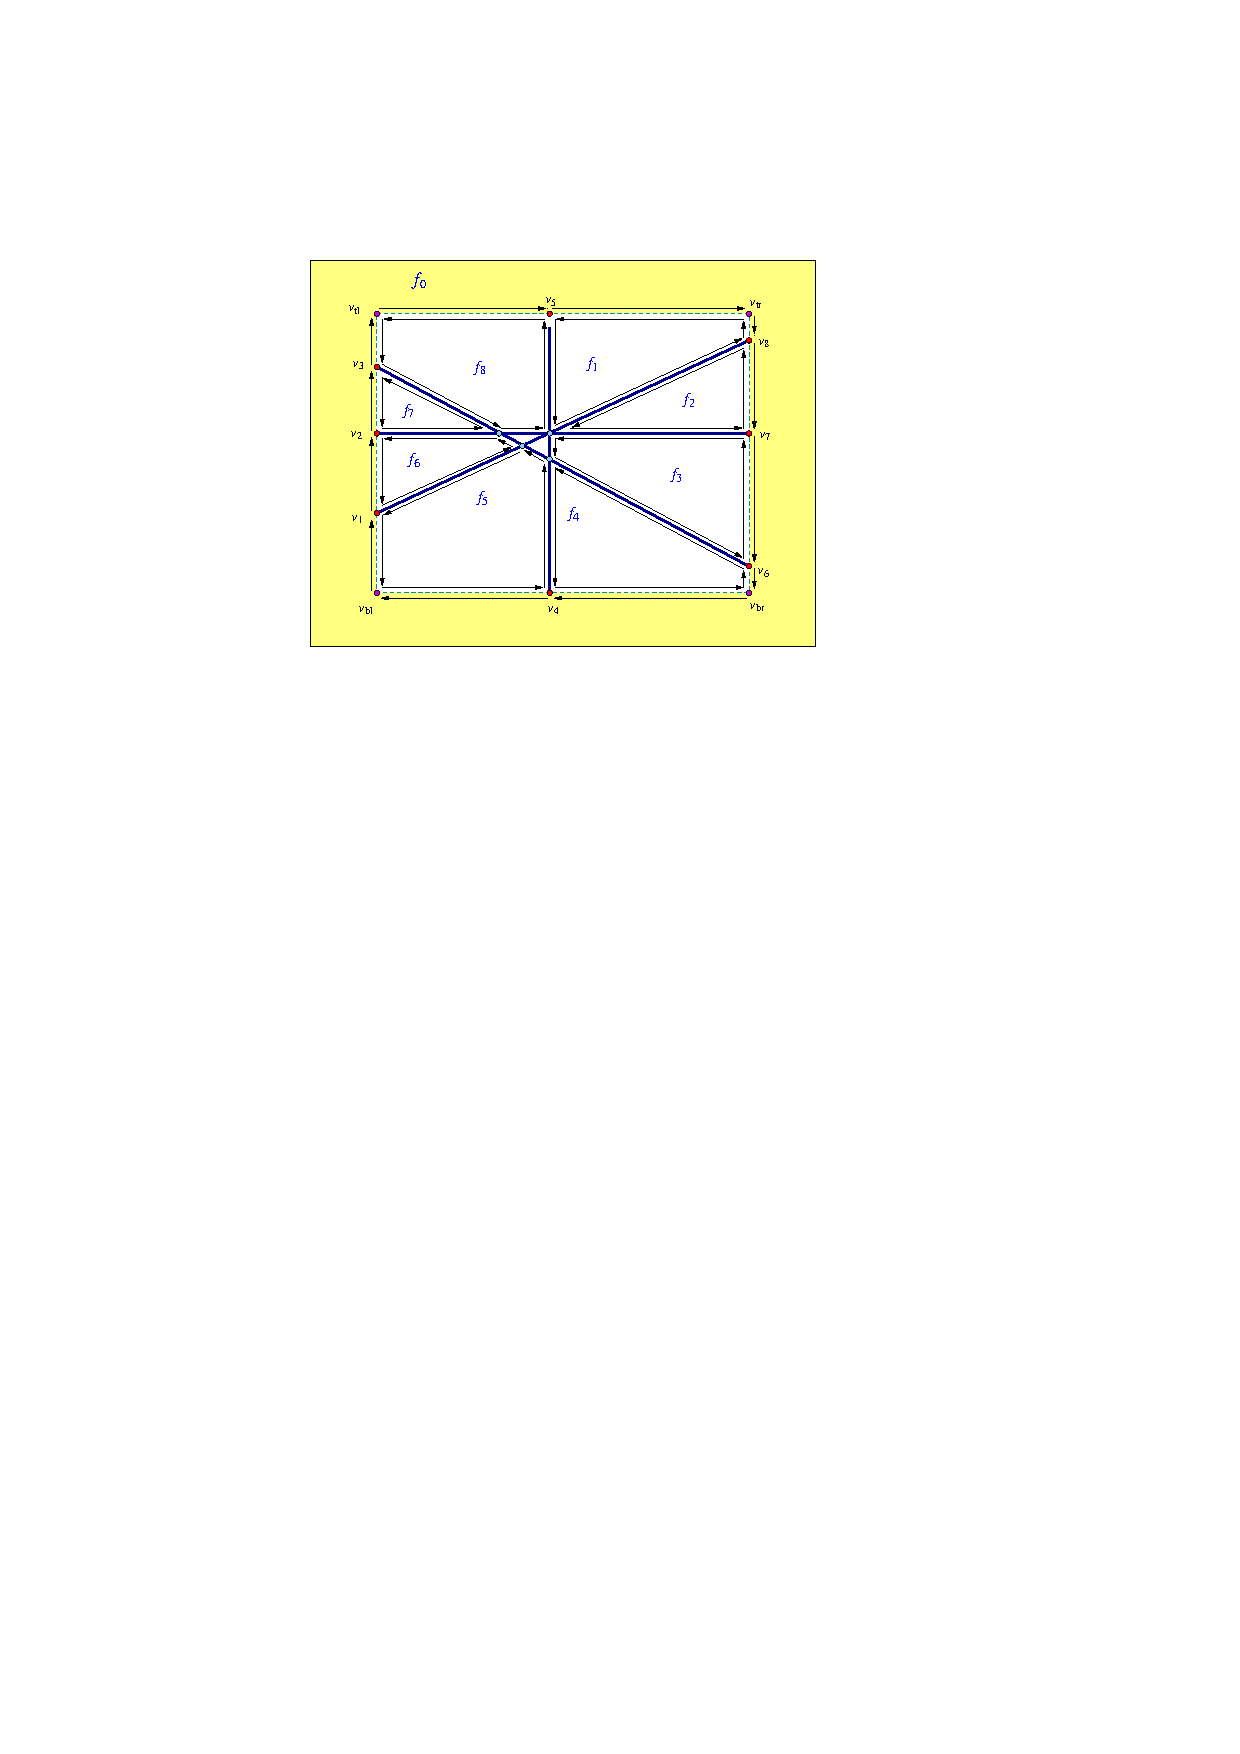
\includegraphics{Arrangement_2/fig/unb_dcel}
  \end{center}
\end{ccTexOnly}
\begin{ccHtmlOnly}
  <p><center>
  <img src="./fig/unb_dcel.gif" border=0 alt="Unbounded DCEL">
  </center>
\end{ccHtmlOnly}
\caption{A \dcel\ representing an arrangement of four lines.
Halfedges are drawn as thin arrows. The vertices $v_1, \ldots, v_8$
lie at infinity and are not associated with valid points. The
halfedges that connect them are fictitious and are not associated
with concrete curves. The face denoted $\tilde{f}$ (lightly shaded)
is the fictitious ``unbounded face'' which lies outside the imaginary
rectangle (dashed) that bounds the actual arrangement. The four
fictitious vertices $v_{\rm bl}, v_{\rm tl}, v_{\rm br}$ and
$v_{\rm tr}$ represent the four corners of the imaginary bounding
rectangle..\label{arr_fig:unb_dcel}}
\end{figure}

Given a set $\calC$ of unbounded curves, a simple approach
for representing the arrangement induced by $\calC$ would be
to clip the unbounded curves using an axis-parallel rectangle that
contains all finite curve endpoints and intersection points among
curves in $\calC$. This process results in a set $\calC$ of bounded
curves (line segments if $\calC$ contains lines and rays), and it is
straightforward to compute the arrangement induced by this set.
However, we would like to operate directly on the unbounded curves
without having to preprocess them. We therefore use an implicit
bounding rectangle embedded in the \dcel\ structure.
Figure~\ref{arr_fig:unb_dcel} shows the arrangement of four lines
that subdivide the plane into eight unbounded faces and two
bounded ones. Notice that in this case the unbounded face have outer
boundaries, and the halfedges along these outer CCBs are drawn as
arrows. The bounding rectangle is drawn in a dashed line. The
vertices $v_1, \ldots, v_8$, which represent unbounded ends of
the foure lines and lie on the bounding rectangle, actually exist at
infinity, and the halfedges connecting them are \emph{fictitious}, and
represent portions of the bounding rectangle. Note that the outer CCBs
of the unbounded faces contain fictitious halfedges. The twins of these
halfedges form together one connected component that corresponds to
the entire imaginary rectangle, which forms a single hole in a face
$\tilde{f}$. We say that $\tilde{f}$ is \emph{fictitious} as it does not
corresponds to a real two-dimensional cell of the arrangement.

Also observe that we have four extra vertices at infinity that are do
not lie on any curve; they are denoted  $v_{\rm bl}, v_{\rm tl},
v_{\rm br}$ and $v_{\rm tr}$, and represent the bottom-left, top-left,
bottom-right and top-right corners of the bounding rectangle,
respectively. By introducing these four fictitious vertices we can
label each of the fictitious edges as lying on the top, the bottom,
the left or the right edge of the imaginary bounding rectangle.
These fictitious edges exists even when the arrangement is empty: in
this case they are connected with four pair of fictitious halfedges,
that define a fictitous face lying inside the imaginary bounding
rectangle and to a single unbounded face.

To summarize, there are four types of arrangement vertices, which
differ from one another by their location on the imaginary bounding
rectangle:
\begin{enumerate}
\item
A ``normal'' vertex, associated with a point in $\real^2$ whose
coordinates are bounded. Such a vertex always lies inside the
bounding rectangle.
\item
A vertex that represent an unbounded end of an $x$-monotone curve
that is defined at $x = -\infty$ or at $x = \infty$. In case of
a horizontal line or a curve with a horizontal asymptote, the
$y$-cooridnate of the curve end may be finite (see for example the
vertices $v_2$ and $v_7$ in Figure~\ref{arr_fig:unb_dcel}), but in
general the curve end also goes to $y = \pm\infty$ (see for instance
the vertices $v_1$, $v_3$, $v_6$ and $v_8$ in
Figure~\ref{arr_fig:unb_dcel}). For our convenience, we will always
take a ``tall'' enough bounding rectangle and treat such vertices as
lying on either the left or right rectangle edges (that is, if a curve
is defined at $x = -\infty$, its left end will be represented by
a vertex on the left edge of the bounding rectangle, and if it is
defined at $x = \infty$, its right end will be represented by a
vertex of the right edge).
\item
A vertex that represent the unbounded end of a vertical line or of a
curve with a vertical asymptote (finite $x$-coordinate and an
unbounded $y$-coordinate). Such a vertex always lies one of the
horizontal edges of the bounding rectangle (either the bottom one if
$y = -\infty$, or the top one if $y = \infty$). The vertices $v_4$
and $v_5$ in Figure~\ref{arr_fig:unb_dcel} are of this type.
\item
The fictitious vertices that represent the four corners of the
imaginary bounding rectangle.
\end{enumerate}
Note that a vertex at infinity of types 1--3 above always has
three incident edges: one concrete edge that is associated with an
unbounded portion of an $x$-monotone curve, and two fictitious edges
connecting the vertex to its neighboring vertices at infinity.
Fictitious vertices (of type 4 above) have exactly two incident edges.
See Section~\ref{arr_sec:traits} on how the traits-class interface
helps imposing the fact that we never have more than one curve
incident to any true vertex at infinity.

\subsection{Basic Manipulation and Traversal Methods\label{arr_ssec:unb_basic}}
%--------------------------------------------

The nested types defined in the \ccc{Arrangement_2} class also
support the following methods, in addition to the ones listed in
Section~\ref{arr_ssec:traverse}:
\begin{itemize}
\item
The \ccc{Vertex} class provides three-valued predicates
\ccc{infinite_in_x()} and \ccc{infinite_in_y()}, which
return \ccc{FINITE} if the vertex has a finite $x$-coordinate (or
$y$-coordinate) and \ccc{MINUS_INFINITY} or \ccc{PLUS_INFINITY} if
the vertex lies at infinity. The Boolean predicate
\ccc{is_at_inifnity()} is also supported, where we can access the
point associated with a vertex only if it is not a vertex at infinity
(recall that a vertex at infinity is not associated with a
\ccc{Point_2} object).
%
\item
The nested \ccc{Halfedge} class provides the Boolean predicate
\ccc{is_fictitious()}. The $x$-monotone curve associated with
a halfedge can be accessed by the \ccc{curve()} method only if the
halfedge is not fictitious.
%
\item
The nested \ccc{Face} class provides the Boolean predicate
\ccc{f.is_fictitious()}. The method \ccc{outer_ccb()} has the
precondition that the face is not fictitious. Note that valid
unbounded faces always have valid CCBs (although this CCB may
comprise only fictitious halfedge in case the arrangement contains
only bounded curves).
\end{itemize}

It is important to observe that the \ccc{arr.number_of_vertices()}
does not count the vertices at infinity. To find out this number
we call \ccc{arr.number_of_vertices_at_infinity()}. Similarly,
\ccc{arr.number_of_edges()} does not count the fictitious edges
(which is always \ccc{arr.number_of_vertices_at_infinity() + 4}) and
\ccc{arr.number_of_faces()} does not count the fictitious face.
The vertex, halfedge, edge and face iterators defined by the
\ccc{Arrangement_2} class only go over true features of the
arrangement --- namely vertices at infinity and fictitious halfedges
and faces are skipped. We mention that the
\ccc{Ccb_halfedge_circulator} of the outer boundary of an unbounded
face or the \ccc{Halfegde_around_vertex_circulator} of a vertex at
infinity do traverse fictitious halfegdes.


\begin{figure}[t]
\begin{ccTexOnly}
  \begin{center}
  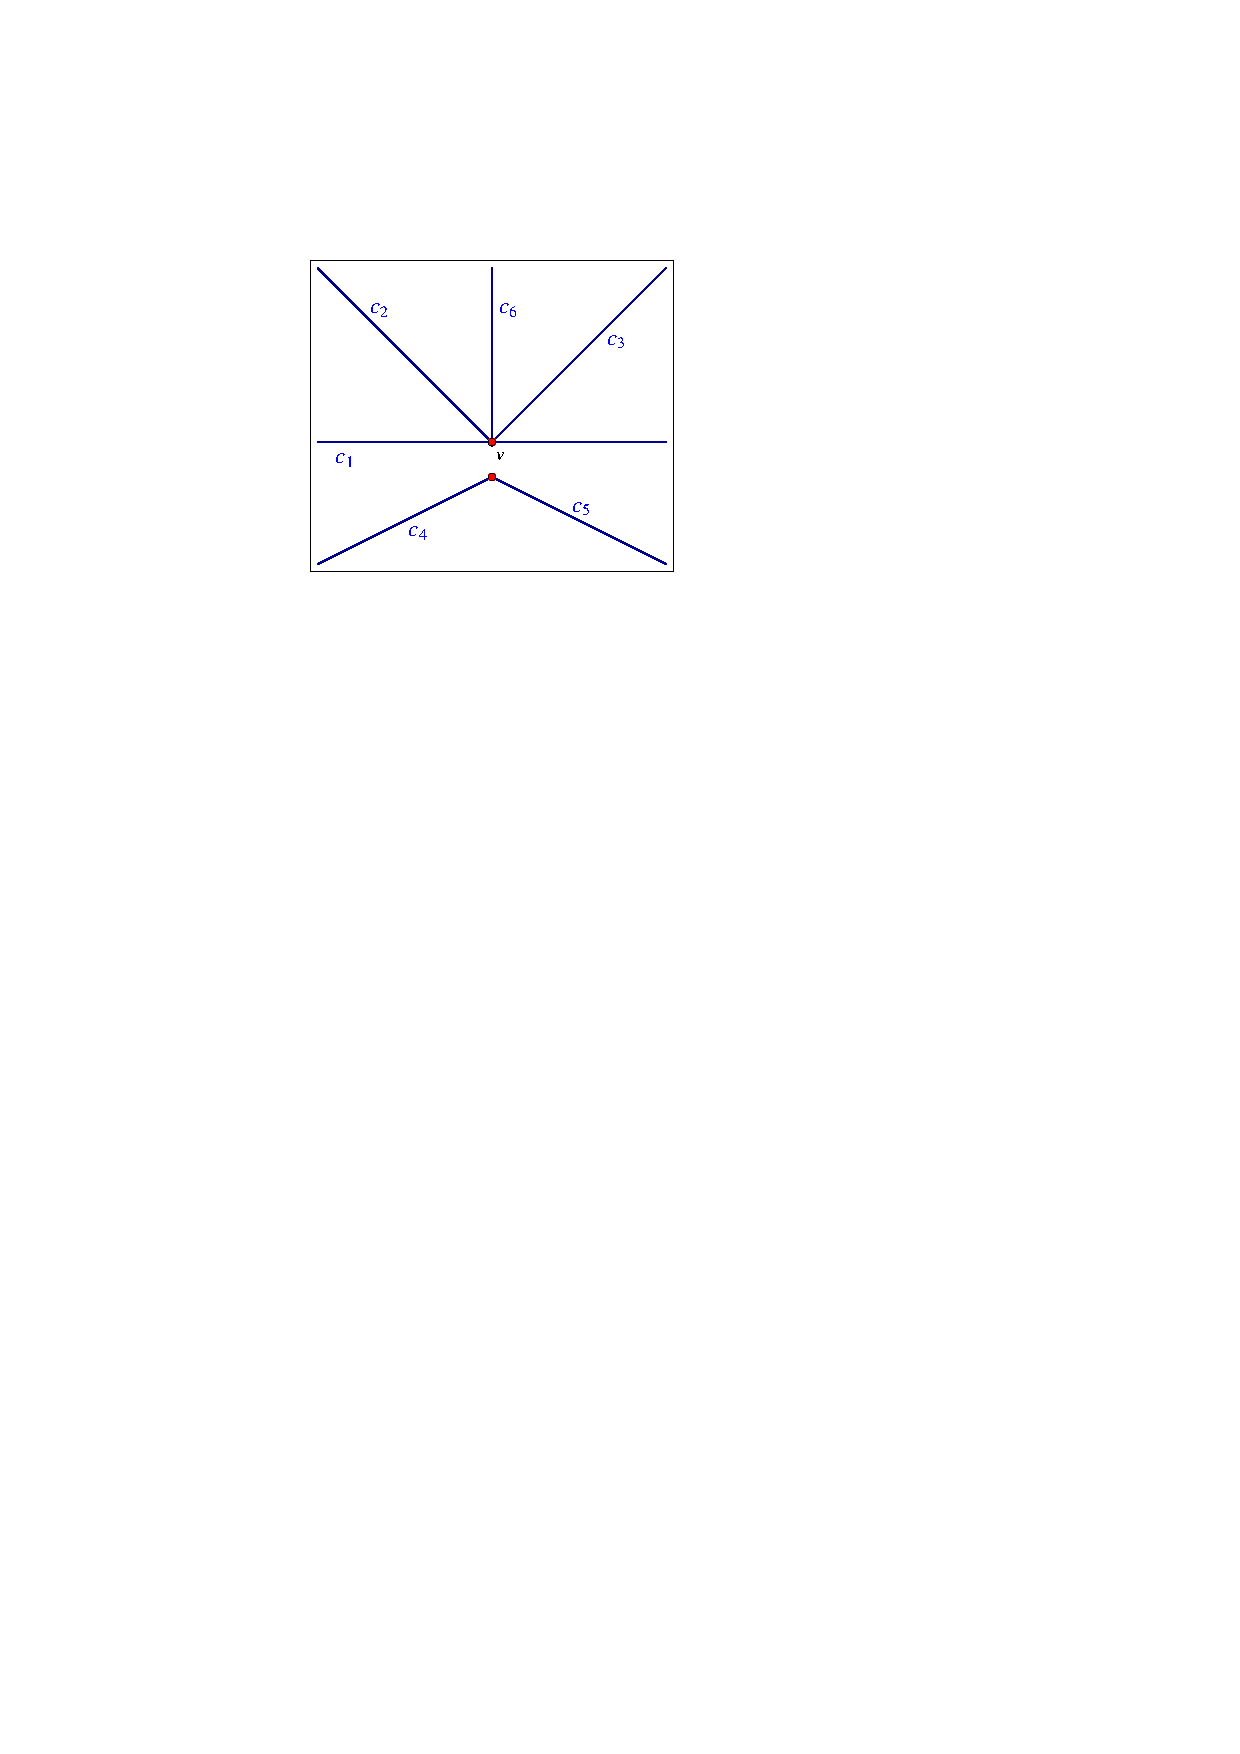
\includegraphics{Arrangement_2/fig/ex_unb1}
  \end{center}
\end{ccTexOnly}
\begin{ccHtmlOnly}
  <p><center>
  <img src="./fig/ex_unb1.gif" border=0 alt="Unbounded example 1">
  </center>
\end{ccHtmlOnly}
\caption{An arrangement of unbounded linear objects, as constructed
in \ccc{ex_unbounded_non_intersecting.C}.\label{arr_fig:ex_unb1}}
\end{figure}

The following example demonstrates the usage of the insertion function
for pairwise interior-disjoint unbounded curves. In this case
we use the traits class \ccc{Arr_linear_traits_2<Kernel>} to
instantiate the \ccc{Arrangement_2} template. This traits class is
capable of representing line segments as well as unbounded linear
curves (namely lines and rays). Observe that objects of the
\ccc{X_monotone_curve_2} type defined by this traits class are
constructible from \ccc{Line_2}, \ccc{Ray_2} and \ccc{Segment_2}
objects, as defined in the kernel.

The first three curves are inserted using the specialized insertion
functions for $x$-monotone curves whose location in the arrangement
is known. Notice that inserting an unbounded curve in the interior
of an unbounded face, or from an existing vertex that represents the
bounded end of the curve, may cause an unbounded face to split (this
is never the case when inserting a bounded curve --- compare with
Section~\ref{arr_sssec:mf_insert_cv}). Three additional rays are then
inserted incrementally, using the insertion function for $x$-monotone
curves whose interior is disjoint from all arrangement features.
Finally, the program prints the size of the arrangement (compare to
the the illustration in Figure~\ref{arr_fig:ex_unb1}) and the outer
boundaries of its six unbounded faces:

\ccIncludeExampleCode{../examples/Arrangement_2/ex_unbounded_non_intersecting.C}

\subsection{Free Functions\label{arr_ssec:unb_global}}
%---------------------------

In principle, all queries and operations that relate to arrangements
of bounded curves can also be applied to arrangements of unbounded
curves. For example, it is possible to issue point-location and
vertical ray-shooting queries (see also Section~\ref{arr_sec:queries})
on arrangements of lines, where the only restriction is that the query
point has finite coordinates.\footnote{Currently, all point-location
strategies except the trapezoidal RIC point-location strategy is
capable of handling arrangements of unbounded curves.} 

In the following example we show how to use the aggregated insertion
function to construct an arrangement of a set of lines. In this
case we read a set of input points from a file (by default we use
\ccc{points.dat}, which contains $100$ points randomly selected
on the grid $[-10000,10000]\times[-10000,10000]$) and determine
whether this set contains at least three collinear points. We solve
this problem by constructing the arrangements of dual lines, where
the line $p^{*}$ dual to the point $p = (p_x, p_y)$ is given by
the equation $y = p_x*x - p_y$, and check whether three (or more)
of the dual lines intersect at a common point by looking for an
arrangement vertex whose degree is greater than $4$. 

\ccIncludeExampleCode{../examples/Arrangement_2/ex_dual_lines.C}

Note that in the \ccc{points.dat} there are no three collinear points.
However, we finally test the algorithm by inserting a line dual to the
midpoint of two randomly selected points into the arrangement and
check that we have created a vertex whose degree is greater than $4$.

